\section{Introduction}

Diesel engines offer several practical benefits, such as lower operating costs and higher fuel efficiency. However,
alongside these advantages, their combustion process produces emissions including unburnt hydrocarbons, carbon monoxide,
nitrogen oxides, and particulate matter, which are hazardous to health and the environment. Some of these pollutants
result from incomplete fuel combustion, combustion of engine lubricating oils and other non-hydrocarbon components,
while others are unavoidable byproducts of the combustion process. To mitigate these pollutants, an aftertreatment
system is installed between the engine outlet and the tailpipe. The diesel engine aftertreatment system comprises
several subsystems, each designed to target specific exhaust pollutants. The Selective Catalytic Reduction (SCR) and
Ammonia Slip Catalysis (ASC) System catalytically reduces nitrogen oxides ($NO_x$) to nitrogen and water vapor. Both SCR
and ASC are constructed as cylindrical bricks, with catalyst coated on the inner surfaces of hollow channels. These
channels are densely arranged to form the brick structure. Multiple SCR catalyst bricks are stacked within a metal
canister (Figure~\ref{fig::aftertreatment_system}), with the ASC brick positioned downstream. The placement and flow
distribution of these components are key design variables.
%============================================================
\begin{figure}[!ht]
    \centering
    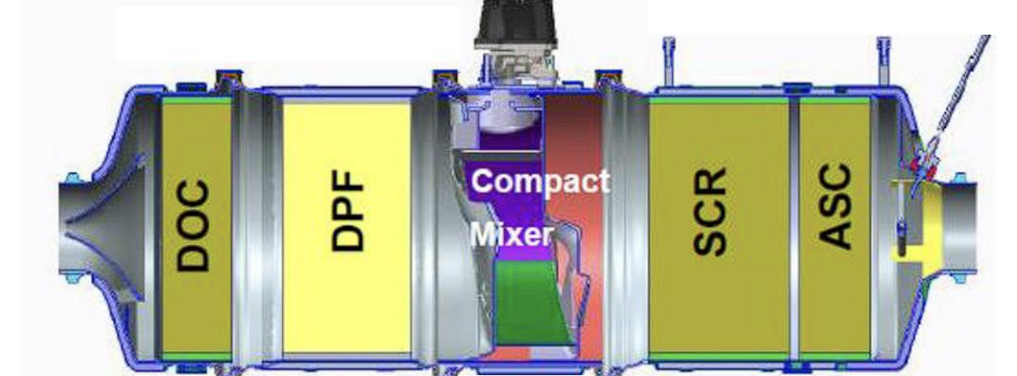
\includegraphics[width=\figWidth]{./figs/1-intro/SCR-ASC_chamber.png}
    \caption{Diesel Aftertreatment System}
    \label{fig::aftertreatment_system}
\end{figure}
% ============================================================
The primary function of the SCR system is to convert engine-out $NO_x$ into nitrogen and water using ammonia derived from
urea dosing, which is adsorbed onto the catalyst. Regulation of this catalytic reduction process aims to minimize
ammonia slip in tailpipe exhaust by two approaches. The first approach employs feedback control, adjusting urea dosing
based on $NO_x$ concentrations at the SCR inlet and tailpipe. The second approach utilizes Ammonia Slip Catalysis, which
oxidizes excess ammonia at the end of the SCR bed (Figure~\ref{fig::exhaust_scheme}).
% ============================================================
\begin{figure}[!ht]
        \centering
        \includegraphics[width=\figWidth]{./figs/1-intro/SCR-ASC_model.png}
        \caption{Schematic of the SCR-ASC System}
        \label{fig::exhaust_scheme}
\end{figure}
% ============================================================
The $NO_x$ reduction capacity of the catalyst diminishes over time due to hydrothermal aging and the accumulation of
contaminants, including excess urea, platinum, sulfur, and phosphorus \cite{matsumoto2016model}. While a robust
urea-dosing controller may attempt to offset catalyst degradation
\cite{chen2016estimation,herman2010diagnostic,hu2018failure} by increasing urea dosing, this strategy can accelerate
aging and further elevate $NO_x$ and ammonia emissions. This has severe environmental and financial implications. Cummins
Inc. had to recall 500,000 medium and heavy-duty trucks in 2018 due to faster SCR catalyst degradation, resulting in
excessive $NO_x$ emissions \cite{jain2023model}. On-board diagnostics (OBD) of SCR catalyst aging under real-world
conditions would help meet increasingly stringent regulations. Some real-world limitations include the unavailability of
ammonia sensors, the unobservability of catalyst state, and $NO_x$ sensor cross-sensitivity to ammonia.

Catalyst aging occurs through several distinct mechanisms, each reducing the concentration of adsorption sites required for catalytic reduction. These mechanisms include:
\begin{inparaenum}[(1)]
\item {Hydrothermal Aging}: Exposure to heat and water vapor from the exhaust leads to irreversible structural and chemical changes on the catalyst surface, reducing ammonia storage capacity \cite{kim2007modeling};
\item {Chemical Deposits}: Deposits of sulfur, phosphorus, and urea-related compounds obstruct active sites for ammonia adsorption, thereby decreasing storage capacity \cite{kim2007modeling};
\item {Platinum Deposits}: Trace amounts of volatilized platinum from the diesel oxidation catalyst (DOC) can accumulate on the front section of the SCR catalyst \cite{toops2010deactivation,jen2009detection}; and
\item {Catalyst Formulation-Specific Aging} \cite{daya2018development,daya2020kinetic}: Examples include dealumination in Fe-zeolite catalysts \cite{toops2010deactivation} and the sintering of anatase $TiO_2$ (higher surface area per mass) to rutile $TiO_2$ (lower surface area per mass) in titanium dioxide-based catalysts \cite{gieshoff2000improved}.
\end{inparaenum}
Furthermore, Catalyst aging is spatially heterogeneous \cite{cheng2007laboratory}. On-engine dynamometer-accelerated
aging results in greater degradation at the front of the catalyst compared to the aft \cite{kim2007modeling}. This
variation is attributed not only to elevated temperatures \cite{toops2010deactivation} but also to the accumulation of
metal and chemical deposits \cite{kim2007modeling}. Cummins' research on high-fidelity aging models
\cite{daya2018development,daya2020kinetic} identifies several types of active sites for ammonia storage, including
Br{\o}nsted acid sites, copper sites, and physisorbed ammonia sites. Two primary sites, S1 and S2, are involved in the
aging process, and their behavior evolves as aging progresses. Mild aging increases S2 while maintaining a constant sum
of S1 and S2, whereas severe aging reduces both S1 and S2. The reaction rates for adsorption and desorption remain
unchanged during mild aging. Standard and fast SCR reactions are largely unaffected by aging \cite{daya2018development}.
The standard reaction predominantly occurs on S1 sites in a fresh catalyst and shifts to S2 sites in an aged catalyst.
Ammonia oxidation increases with aging on S2 sites. Therefore, it can be concluded that aging primarily reduces the
concentration of adsorption sites while preserving similar reaction kinetics.

On-board aging diagnostics for SCR-ASC systems are categorized as intrusive or non-intrusive. Intrusive diagnostics
require intervention in the catalyst's normal operation, using controlled excitation \cite{herman2010diagnostic} of
specific system dynamics and comparing the resulting responses to a known reference
\cite{pezzini2009methodology,hu2017improving}. Non-intrusive diagnostics, by contrast, assess the aging state without
actively modifying system inputs. This approach involves a dynamic model for the system that is consistent with the observed data.

% ============================================================
\subsection{SCR-ASC Modelling: State of the Art}
A deductive approach to aging diagnostics models the dynamics of the signal-generating system, specifically the SCR-ASC
system, and incorporates aging effects by tracking changes in selected model parameters. Numerous studies have addressed
the modelling and control of SCR-ASC systems \cite{yuan2015diesel}. A common modelling strategy involves approximating
the partial differential equation (PDE) model for the plug flow reaction as a set of ordinary differential equations
(ODEs) using a series of Continuously Stirred Tank Reactors (CSTRs) \cite{hsieh2011development,nova2014urea}. The number
of CSTRs implemented often serves as an indicator of model fidelity. For instance,
\cite{chen2016estimation,ma2017observer,devarakonda2009model,hsieh2011development} employ four-cell CSTR models,
\cite{hu2018failure,hu2017improving,stadlbauer2015adaptive,schar2004control} utilize three-cell models, and
\cite{jiang2019hydrothermal,upadhyay2002modeling,devarakonda2008adequacy} adopt two-cell models. The single CSTR
approach was initially justified in \cite{devarakonda2008adequacy}, where a nonlinear model was developed based on these
assumptions and subsequently linearized for feedback control design \cite{devarakonda2009model}. Observers have been
developed to estimate the states associated with catalyst storage \cite{ma2017observer,jain2020term}. A method for
detecting catalyst aging by observing changes in the catalyst's maximum storage capacity, modelled as an exponential
function of temperature, was also introduced in \cite{ma2017observer,jiang2019hydrothermal}. Additionally, an on-board
diagnostics (OBD) approach for catalyst aging, utilizing tailpipe $NO_x$ and ammonia measurements, was proposed in
\cite{matsumoto2016model}. This method is based on the hypothesis of reduced adsorption sites and has been demonstrated
on real-world trucks.

A persistent challenge in these studies is that system identification leads to a nonconvex, nonlinear parameter
estimation problem. Moreover, many approaches assume the availability of all gaseous states at the tailpipe for state
estimation and to mitigate cross-sensitivity effects in $NO_x$ sensors. This assumption is not valid in practical
applications, as tailpipe ammonia measurements are generally unavailable in commercial vehicles. Another notable
limitation of the CSTR model, regarding sensor sampling, is that its discretization does not consider reactant residence
time, which results in impractically high sampling frequencies. Furthermore, accurate discretization requires at least
two CSTRs to adequately capture system dynamics and causality \cite{charla2024reduced}, thereby increasing the model
order. The remainder of the section presents the CSTR model based on the three principal reactions and examines its
limitations.

\subsubsection{Continuous Stirred Tank Reactor Model}
\begin{figure}[!ht]
    \centering
    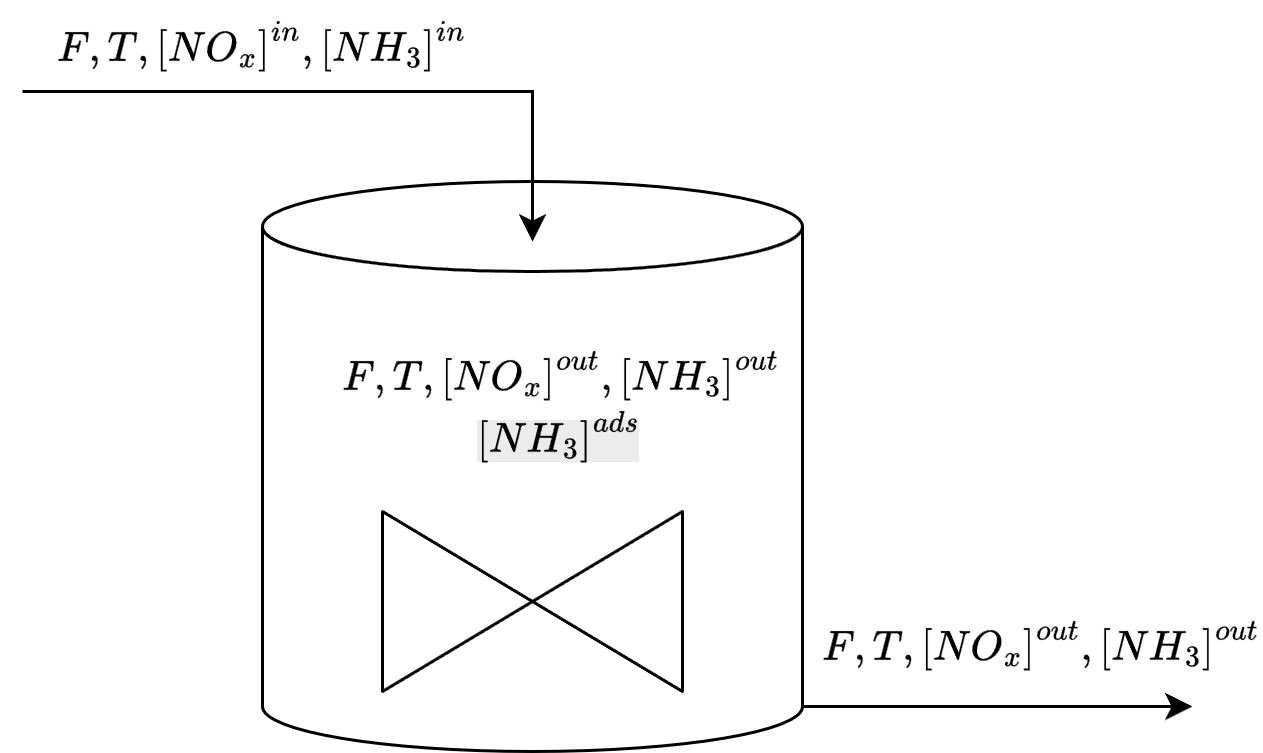
\includegraphics[width=\figWidth]{./figs/1-intro/CSTR.png}
    \caption{Schematic of CSTR model for SCR-ASC System}
    \label{fig::cstr_schematic}
\end{figure}
The model development is based on specific assumptions that reflect typical operating conditions and system behavior.
The CSTR assumption underpins the construction of the reaction flow model for SCR reactions. Drawing on reduced-order
modelling results from previous studies, including \cite{devarakonda2008adequacy,jain2023diagnostics}, the
number of reactions considered is reduced from the full set to three (Table~\ref{tab::react_rates}). The analysis
focuses exclusively on the standard SCR reaction, with the assumption that all $NO_x$ in the exhaust gas is $NO$, since
commercially available $NO_x$ sensors cannot differentiate between $NO$ and $NO_2$ \cite{nova2014urea}. The slow SCR
reaction is omitted, as the exhaust flow rate ensures it does not significantly affect the concentration of tailpipe
exhaust components. Mass transfer is neglected, indicating that the catalyst's chemical kinetics are reaction controlled
because the standard SCR reaction rate exceeds the exhaust fluid flow rate. A $100\%$ nitrogen selectivity for ammonia
oxidation is assumed for both SCR and ASC \cite{jain2023diagnostics}. Furthermore, the reaction rates are assumed to
depend solely on the gas-phase concentrations of $NO_x$, $NH_3$, the adsorbed ammonia, and the available adsorption
sites.
\begin{table}[!ht]
    \begin{center}
    \caption{SCR-ASC Reactions and Rates Considered for Model Development}
    \label{tab::react_rates}
    \begin{tabular}{|l|c|l|}
        \hline
        Reaction & Reaction Equation & Reaction Rate \\ \hline
        % ====
        Standard SCR &
        $4 NH_3 ^{(ads)} + 4 NO + O_2 \longrightarrow 4 N_2 + 6 H_2O$ &
        $r_{scr} = k_{scr} \con{NO_x}^{out} \con{NH_3}^{ads}$ \\ \hline
        % =======
        AMOX &
        $4 NH_3 + 3 O_2 \longrightarrow 2 N_2 + 6 H_2O $ &
        $r_{ox} = k_{ox} \con{NH_3}^{out}$ \\ \hline
        % =======
        Adsorption&
        $NH_3 + \theta_{free} \longrightarrow NH_3(ads)$ &
        $r_{ads} = k_{ads} \con{NH_3}^{out} \lr{\Gamma - \con{NH_3}^{ads}}$ \\ \hline
        %=======
        Desorption &
        $NH_3 ^{(ads)} \longrightarrow NH_3 + \theta_{free}$ &
        $r_{des} = k_{des} \con{NH_3}^{ads}$ \\ \hline
    \end{tabular}
    \end{center}
    *$\Gamma$ is the total adsorption site concentration.
\end{table}

In continuous stirred-tank reactors (CSTRs), reaction rates are governed by outlet concentrations, as defined by
reaction rate expressions. This relationship arises from the uniform mixing assumption at steady state: fluid with a
specified inlet concentration enters the CSTR, undergoes complete mixing, and reacts, resulting in outlet concentrations
that match those within the reactor (Figure~\ref{fig::cstr_schematic}). When a plug-flow reactor is modelled as a single
CSTR, the causality of the reaction rates is reversed. Employing multiple CSTRs introduces intermediate states, which
alleviates the impact of this causality reversal. As a result, a valid CSTR model generally contains more states than
can be measured, making the system unobservable. This limitation is one of the two key motivations behind the discrete
nonlinear model developed in this thesis.

One additional consideration is the saturation of adsorption sites on the catalyst surface. The total concentration of adsorption sites, denoted as $\Gamma$, is the sum of occupied and free adsorption sites. Thus, at any given time,
\begin{align}
    \Gamma \geq \con{NH_3}^{ads} \geq 0
\end{align}
Thus, the system dynamics are conditioned on the saturation state of the catalyst. This phenomenon is captured in the model through the following switching function:
\begin{align}
    g_{sat} \lr{\sigma} = \begin{cases}
        \sigma & \text{if } 0 \leq \sigma \leq \Gamma \\
        \Gamma & \text{if } \sigma > \Gamma \\
        0 & \text{if } \sigma < 0
    \end{cases}
    \label{eqn::g_sat}
\end{align}
We have dynamics of the concentration of reactants from the mass balance for the CSTR \cite{hsieh2011development}:
\begin{align}
    V_{scr} \dot{\con{NO_x}}^{out} &= F_{vol} \lr{\con{NO_x}^{in}-\con{NO_x}^{out}} - V_{scr} \lr{k_{scr} \con{NO_x}^{out} g_{sat}\lr{\con{NH_3}^{ads}}} \label{eqn::nox_mass_bal}\\
    % ====
    V_{scr} \dot{\con{NH_3}}^{out} &= F_{vol} \lr{\con{NH_3}^{in}-\con{NH_3}^{out}} \notag \\
    & \quad  + V_{scr}\lr{ - k_{ads} \con{NH_3}^{out} \lr{\Gamma - g_{sat}\lr{\con{NH_3}^{ads}}} + k_{des} g_{sat}\lr{{\con{NH_3}^{ads}}}} \label{eqn::nh3_mass_bal}
    \\
    % ====
    \dot{\con{NH_3}}^{ads} &= k_{ads} \con{NH_3}^{out} \lr{\Gamma - g_{sat}\lr{\con{NH_3}^{ads}}}
                            - k_{des} g_{sat}\lr{{\con{NH_3}^{ads}}} \notag \\
                            & \qquad - k_{scr} \con{NO_x}^{out} g_{sat}\lr{\con{NH_3}^{ads}} \label{eqn::nh3_ads_mass_bal}
\end{align}
The actual input to the system is urea (AdBlue ($32.5\%$ aqueous urea solution) \cite{nova2014urea})
injection that is converted to ammonia. This can be modelled by the following equation~(\ref{eqn::urea_inj}).
\begin{equation}{\label{eqn::urea_inj}}
    \dot{\con{NH_3}}^{in} = \frac{1}{\tau_{urea}} \lrf{ - \con{NH_3}^{in} +   \frac{b_{urea}}{F_{vol}}  u_{inj}}
\end{equation}
The four equations presented constitute the nonlinear state-space model for the SCR-ASC system under the single CSTR
assumption. However, this model lacks parsimony and identifiability given the current measurement set. To obtain an
identifiable model, the nonlinear system can be linearized, and lumped parameters for input-output equations can be
derived based on the available measurements~\cite{charla2024reduced}.

Furthermore, the hybrid dynamics modelled in the above equations capture the high-frequency reaction kinetics coupled
with mass flow. The slowest process, or dominant mode, can be approximated as a first-order system with residence time
as the time constant. For effective sampling of such a system, the sampling frequency should be n-times (at least twice)
the inverse of the residence time. Let $\tau$ be the residence time of the reacting flow through the SCR-ASC system,
then the sampling frequency $f_s = 1/t_s$ should be:
\begin{align}
    f_s &\geq \frac{n}{\tau}
    \implies t_s \leq \frac{\tau}{n} \qquad n \geq 2
\end{align}
Thus, the CSTR model is valid only for high sampling frequencies. If we plot the residence time on the y-axis and the
sampling time on the x-axis, the valid region for the CSTR model lies in the shaded area of
Figure~\ref{fig::mdl_validity}. The above analysis highlights the limitations of the CSTR model in practical applications, particularly regarding
sampling frequency requirements. This insight further motivates the development of alternative modelling approaches that
can accommodate lower sampling frequencies while still accurately capturing the dynamics of the SCR-ASC system.


The sensor limitations and identifiability requirements outlined in previous chapters necessitate the development of a
dynamic model for the SCR-ASC system. This model must possess parameters that are identifiable from sensor data and
exhibit dynamics within the frequency range captured by the sensors. Accordingly, the model's validity region in the
$\tau-t_s$ (residence time versus sampling time) plane should encompass the decimated test-cell and truck data residence
times (Figure~\ref{fig::res_samp_plane}). $\tau-t_s$ plane is the plot of the mode of the residence time versus sampling
time for a given test-cell or truck data. This representation indicates the similarity between data sets in terms of the
frequency content of their captured dynamics. Therefore, this chapter proposes a discrete nonlinear state-space model
for the SCR-ASC dynamics that alternates between catalyst saturation and unsaturation states.

\begin{figure}[!ht]
        \centering
        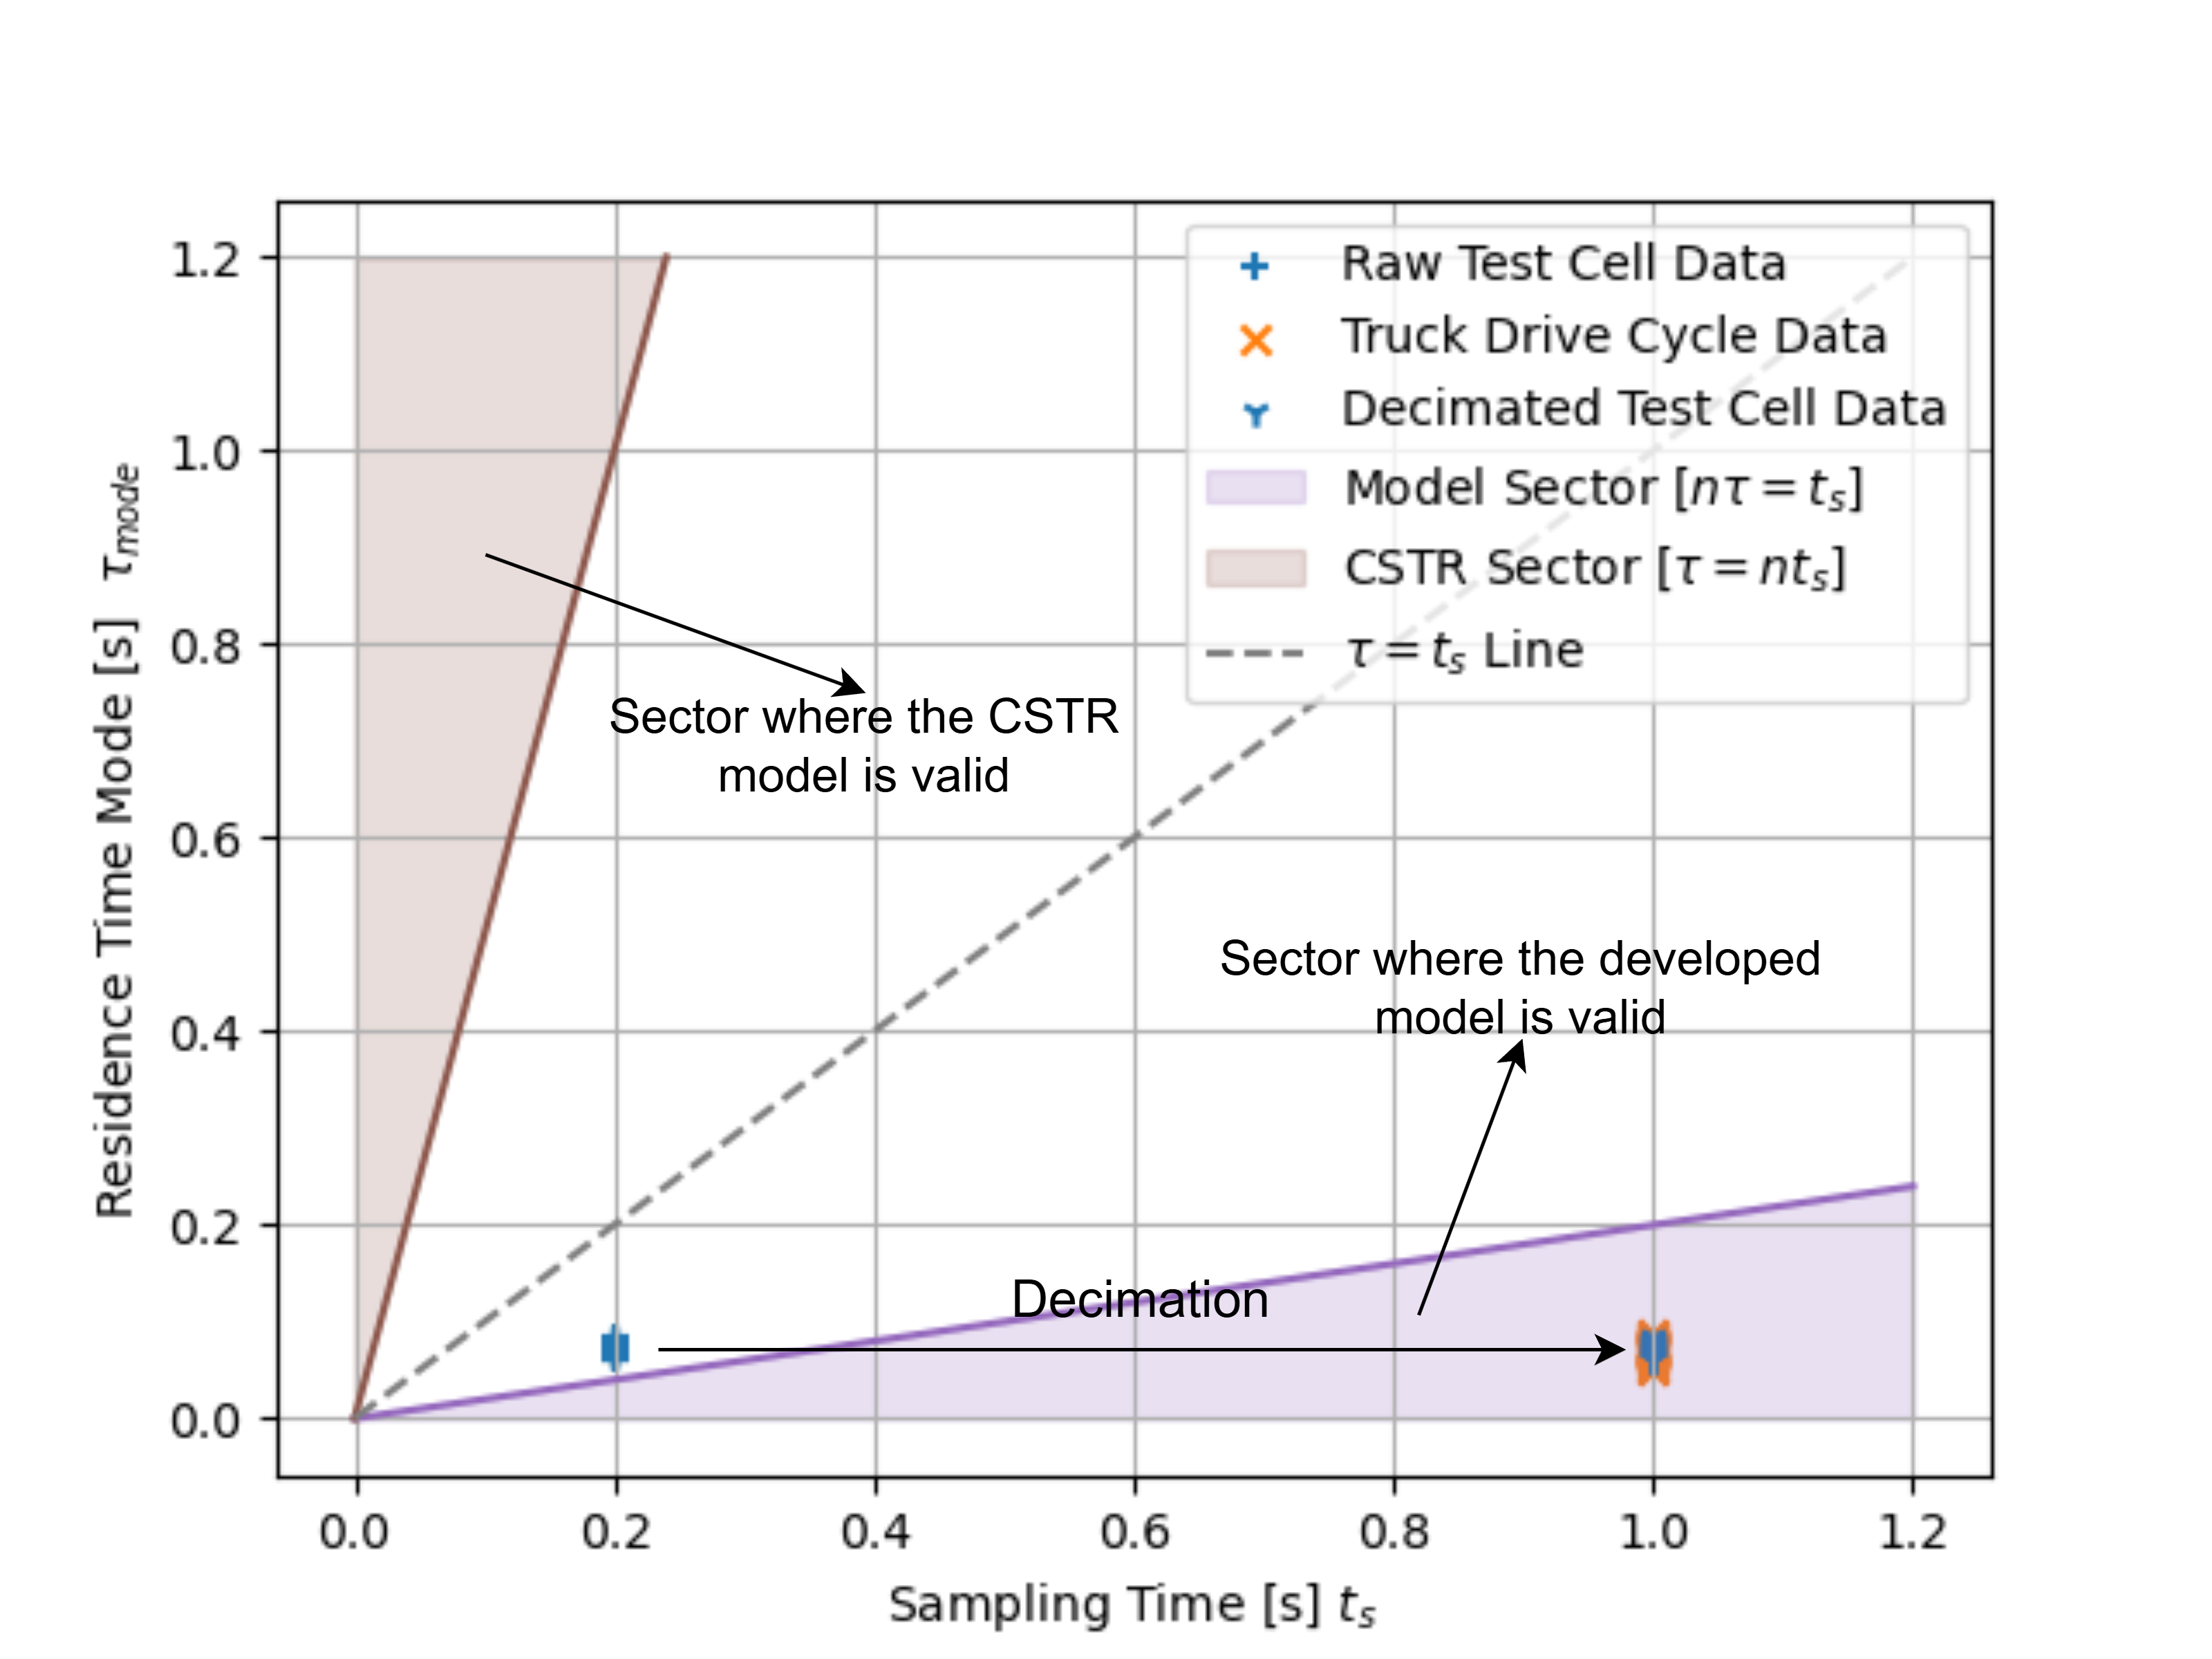
\includegraphics[width=\figWidth]{./figs/1-intro/mdl_valid.png}
        \caption{Validity region of the discrete nonlinear switched model for SCR-ASC dynamics}
        \label{fig::mdl_validity}
\end{figure}

The model development employs a control volume approach, formulating molar conservation equations for the reacting
species between the inlet and outlet. The primary innovation involves integrating these conservation equations over the
residence time and summing them telescopically according to the number of residence times occurring within a single
sampling period. This methodology explicitly incorporates both residence time and sampling time into the model.

The chapter begins by detailing the reactions occurring within the SCR-ASC system and outlining the assumptions adopted
to reduce model order while maintaining identifiability, causality, and parsimony. Dynamic equations for each reacting
species are then derived using this approach, with all assumptions explicitly stated and justified. The resulting
nonlinear state-space model for the SCR-ASC system is subsequently presented. The transformation of this nonlinear model
into an identifiable input-output model, along with the parameter estimation algorithm and model validation, is
addressed in the following chapter.
